\section{Accessibilità}

\paragraph{Linee guida}

Come sono stati impostati i testi alternativi alle immagini
%TODO
The alt attribute should typically:
Be accurate and equivalent in presenting the same content and function of the image.
Be succinct. This means the correct content (if there is content) and function (if there is a function) of the image should be presented as succinctly as is appropriate. Typically no more than a few words are necessary, though rarely a short sentence or two may be appropriate.
NOT be redundant or provide the same information as text within the context of the image.
NOT use the phrases "image of ..." or "graphic of ..." to describe the image. It usually apparent to the user that it is an image. And if the image is conveying content, it is typically not necessary that the user know that it is an image that is conveying the content, as opposed to text. If the fact that an image is a photograph or illustration, etc. is important content, it may be useful to include this in alternative text.

\subsection{Accessibilità sezione pubblica}

\paragraph{Cecità ai colori}
Per testare che il sito sia accessibile alle persone daltoniche, tetracromiche o con altri problemi riguardanti i colori si è utilizzato l'estensione Vischeck, scaricabile dal sito Vischeck.com. Tale estensione, eseguibile con ImageJ, data un'immagine o una pagina web, mostra come viene percepita da chi soffre di cecità ai colori. È bastato verificare un paio di pagine, in quanto i colori e le immagini di background utilizzate sono le medesime in tutte le pagine.

\begin{figure}[H]
		\centering 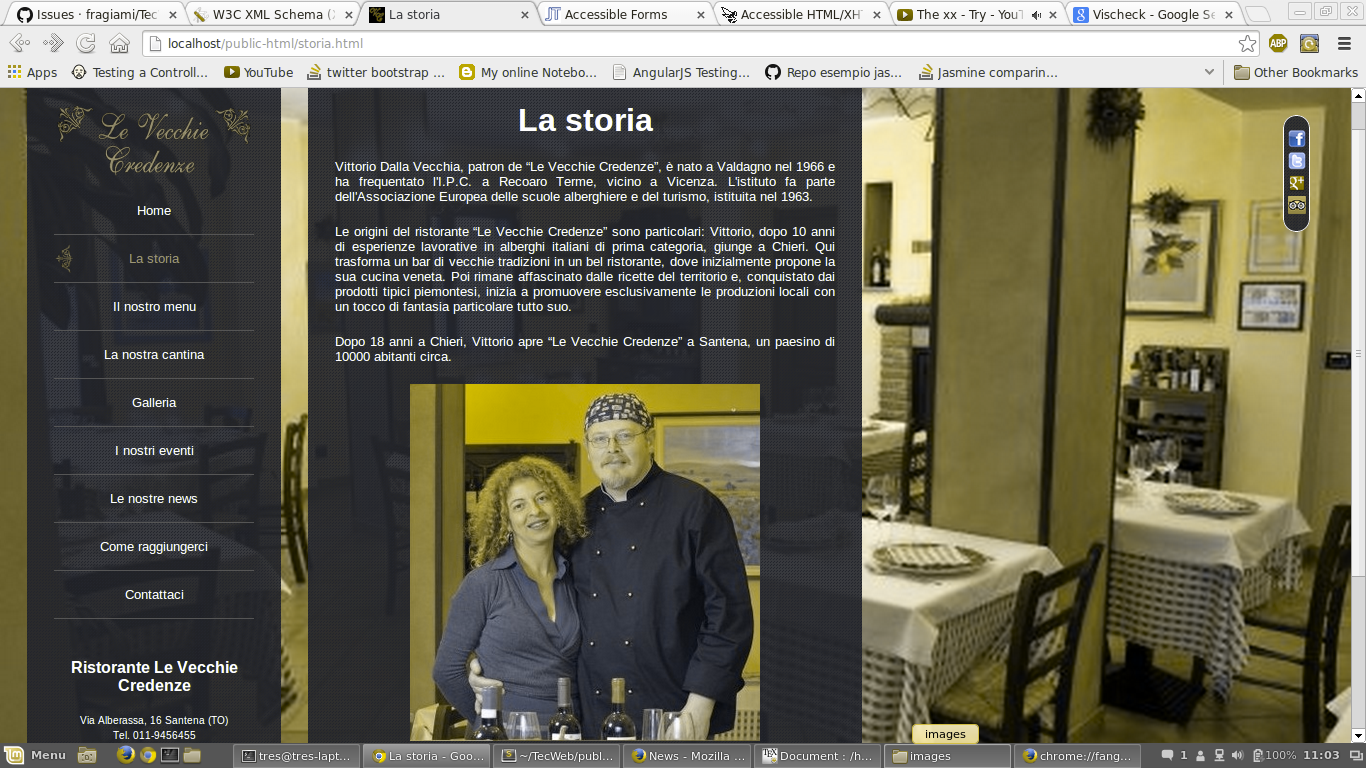
\includegraphics[width=0.8\textwidth]{images/color1.png}
		\caption{Esempio di pagina vista da chi soffre di deuteranopia}
\end{figure}
	
\begin{figure}[H]
		\centering 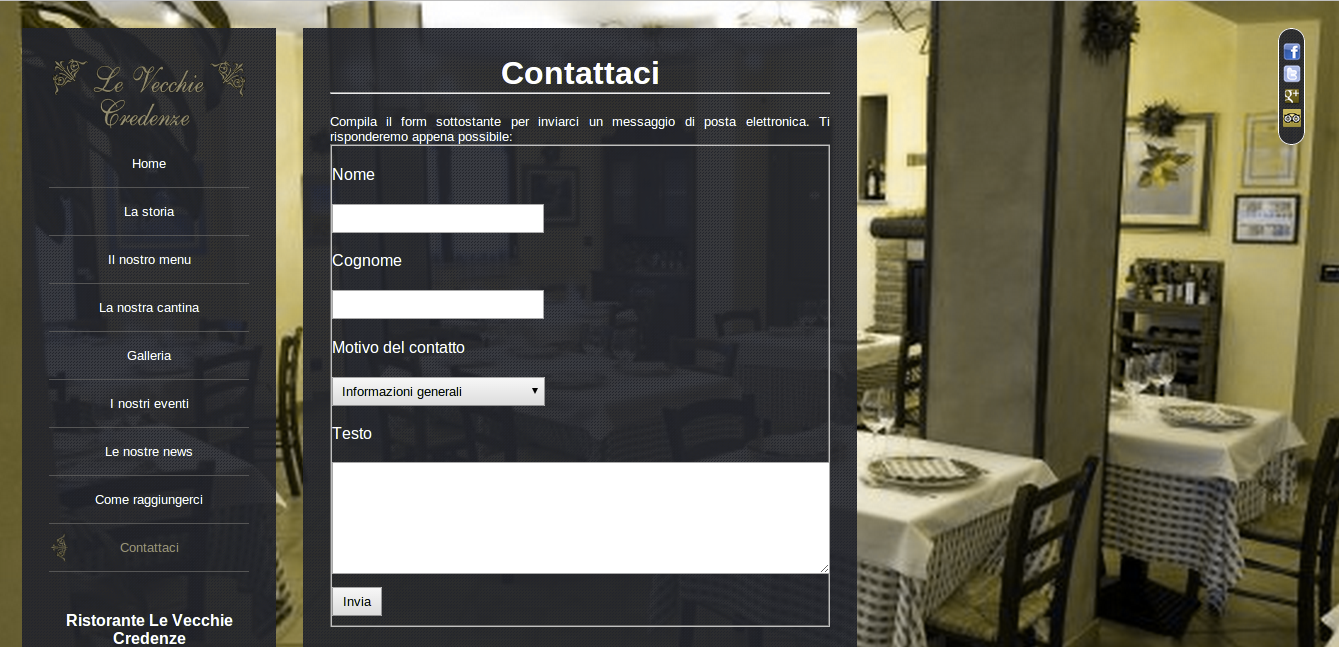
\includegraphics[width=0.8\textwidth]{images/color2.png}
		\caption{Esempio di pagina vista da chi soffre di protanopia}
\end{figure}
	
\begin{figure}[H]
		\centering 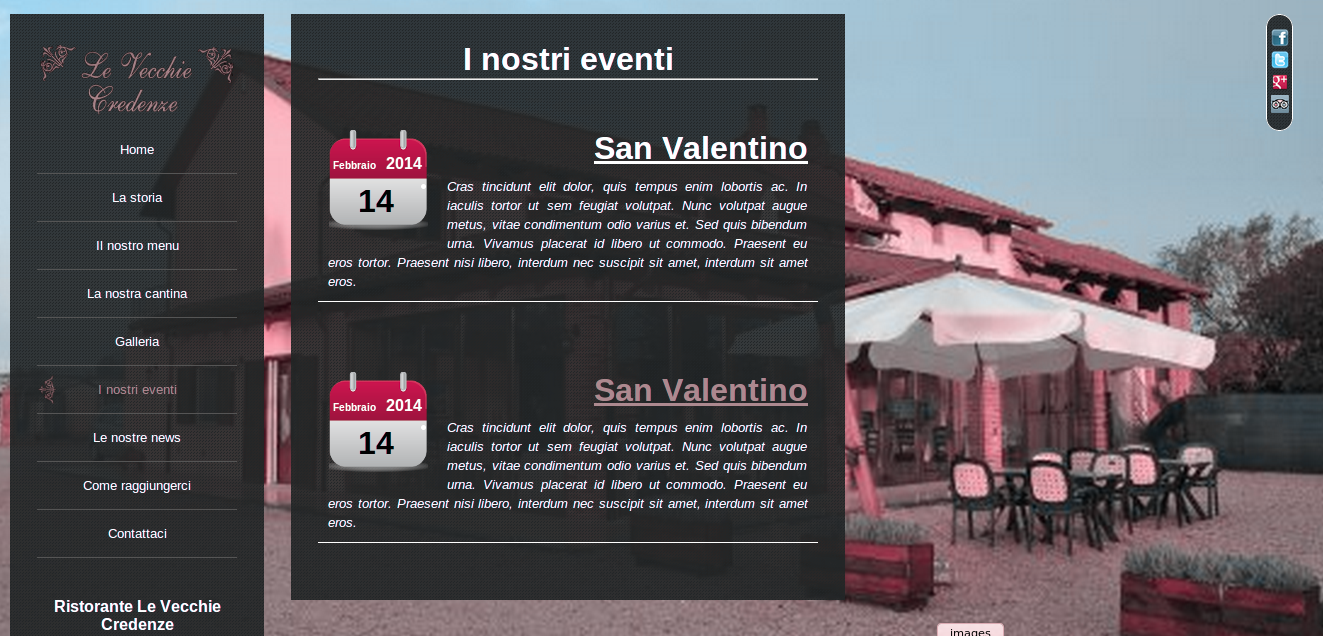
\includegraphics[width=0.8\textwidth]{images/color3.png}
		\caption{Esempio di pagina vista da chi soffre di tritanopia}
\end{figure}


\paragraph{Utilizzo della sola tastiera}
Per essere accessibile un sito deve poter essere navigabile utilizzando solamente la tastiera. 
Ogni pagina è stata testata ed il risultato è che l'intero sito è navigabile utilizzando \emph{Tab} ed \emph{Enter}.
Non sono stati utilizzati gli attributi \emph{tabindex} per i link in quanto il flusso logico del sito è semplice e lineare.

\paragraph{Cecità}
Per testare il sito rispetto agli \emph{screen reader} è stata utilizzata l'estensione \emph{Fangs} del browser Firefox.
Tale estensione simula come un generico screen reader interpreta le varie pagine. 
Un problema che è sorto è stata la mancanza dell'italiano tra le lingue supportate da Fangs. Nonostante ogni pagina indichi l'italiano come lingua di default, tramite l'attributo \emph{lang}, Fangs imposta l'inglese come lingua di default, e ad esempio legge i numeri decimali come centinaio (Ecco nella pagina cantina 2,00 diventa two hundred).

Nonostante ciò Fangs ha permesso di verificare che:
\begin{itemize}
\item tutti i link vengano catturati, e che ogni link abbia un significato chiaro;
\item cambi lingua, le abbreviazioni e le tabelle fossero gestiti correttamente;
\item visualizzare gli headers della pagina, funzionalità offerta da alcuni scree reader e utile per capire a grandi linee il contenuto della pagina e la sua struttura. Un esempio dell'utilità di tale funzionalità è data dalla pagina news, in cui grazie agli header è possibile accedere immediatamente ai titoli di tutte le news presenti, per poi selezionare quella di proprio interesse.s
\item Ogni immagine abbia il rispettivo testo alternativo.
\end{itemize} 

\begin{figure}[H]
		\centering 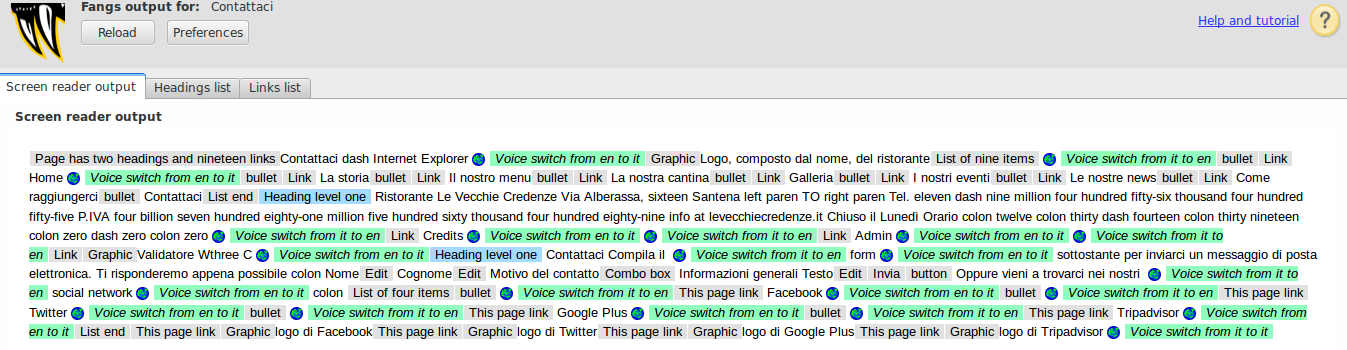
\includegraphics[width=0.8\textwidth]{images/fangs.png}
		\caption{Output di Fangs}
	\end{figure}
	
	\begin{figure}[H]
		\centering 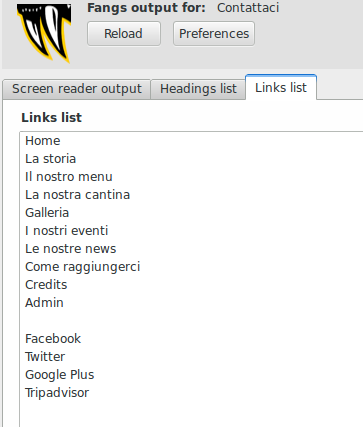
\includegraphics[width=0.8\textwidth]{images/fangsLink.png}
		\caption{Elenco di link della pagina, come visualizzati da Fangs}
	\end{figure}

\paragraph{Accessibilità dei form}

Possiamo vedere un esempio di accessibilità dei form nella pagina contatti.html.

Per chi utilizza uno screen reader, nel compilare un form è fondamentale sapere come compilare gli input. Per questo motivo ad ogni \emph{input type text} è associata una label con attributo for, il cui valore è l'id dell'input a cui fa riferimento. Con questa tecnica lo screen reader sa certamente collegare nel modo corretto un'input alla sua label.
Tale tecnica è stata utilizzata anche per i \emph{select menus}

Per ogni bottone è stato utilizzato il tipo submit in quanto button necessita che javascript sia bilitato per funzionare, inoltre in ogni bottone è stato valorizzato l'attributo value, in modo che lo screen reader dia un significato esplicito all'azione del bottone.

\paragraph{Total Validato}
Total validator è uno strumento, che tramite un'apposita estensione di Firefox permette di verificare l'accessibilità di una pagina web secondo alcuni parametri.
Le impostazioni di total validator scelte sono le più stringenti, richiedendo un'accessibilità aderente allo standard WCAG 2.0 AAA


\subsection{Accessibilità sezione amministrazione}

i form obbligatori sono chiaramente identificati

Inserire la star, e includere immagine screenReaderRequiredForm.png

Dovresti dimostrare che il sito è ok per i daltonici etc, utilizzabile con la sola tastiera (navigare tra i link, compilare form etc) e easy da usare con uno screen reader. E deve essere a nche a prova di idiota.